\chapter{Literature Review}
\label{ch:literature}
This chapter reviews the scientific literature relevant to interaction-point
perception in hospital environments, with a focus on instance segmentation,
dataset design, annotation strategies, and deployment of computer-vision models
on embedded systems.

\section{Perception of human-machine interaction elements}

Human--machine interaction elements such as elevator buttons, door panels, and
access readers are important targets for indoor service robots operating in
hospital environments. Previous work in healthcare and service robotics shows
that reliable interaction with such infrastructure is required for autonomous
operation across multiple floors and restricted areas
\citep{holland2021servicerobots,masala2025assistiverobotics}.

From a computer-vision perspective, these interaction elements are challenging
to detect because they are small, visually similar, and often arranged closely
together on control panels. Studies on visual perception for robotic interaction
report that elevator panels typically contain many buttons with minimal visual
differences, which makes robust localization difficult under varying lighting
conditions, reflections, and viewing angles \citep{bernard2020interfaces}.

General indoor-robot perception systems often focus on detecting large objects
or structural elements and assume that interaction with building infrastructure
is externally supported or environment-specific. However, research on autonomous
service robots emphasizes that scalable deployment requires perception systems
that can directly identify actionable interface elements from camera and sensor data,
without relying on prior knowledge of the environment
\citep{wang2019indoorrobots}.

These findings indicate that interaction-point perception is a fine-grained
vision problem in which individual button instances on a panel must be localized
accurately within visually dense scenes. At the same time, the cited studies
mainly motivate the problem rather than solving it under the embedded and
deployment-oriented constraints of this project. This observation motivates the
need for vision methods that go beyond coarse detection of panels or regions and
instead support precise identification of individual button instances.


\section{Formulating interaction-point perception as a vision problem}

Vision-based perception problems in robotics are commonly formulated as image
classification, object detection, or semantic segmentation tasks. Each formulation
implies different assumptions about the structure of the scene and the required
output, which directly affects suitability for robotic interaction.

Image classification assigns a single label to an entire image and is therefore
unsuitable for scenarios where multiple interaction elements appear simultaneously.
Object detection extends this formulation by predicting bounding boxes and class
labels for individual objects; in this project, those objects correspond to
individual button instances on an elevator panel. While detection-based approaches have been widely
used for indoor perception tasks, bounding boxes provide only coarse spatial
localization and do not capture the precise shape of interaction elements
\citep{ren2015fasterrcnn,redmon2016yolo}.

Semantic segmentation addresses this limitation by assigning a class label to
each pixel in the image. Formally, semantic segmentation can be expressed as a
pixel-wise classification function
\[
f_{\theta} : \mathbb{R}^{H \times W \times C} \rightarrow \{1,\dots,K\}^{H \times W},
\]
where $H$ and $W$ denote image height and width, $C$ the number of input channels,
and $K$ the number of semantic classes \citep{long2015fcn}. Although this formulation
enables precise localization, all pixels belonging to the same class are treated
as a single region. As a result, semantic segmentation cannot distinguish between
multiple instances of the same object class.

For interaction-point perception, this limitation is critical. Elevator panels
often contain many visually similar button instances, each corresponding to a
distinct action \citep{bernard2020interfaces}. By definition, semantic
segmentation assigns a class label to each pixel but does not separate
same-class instances \citep{long2015fcn}, whereas instance segmentation
predicts a separate mask for each detected instance \citep{he2017maskrcnn}. For an
elevator panel, a semantic segmentation output would therefore label button
pixels by class without separating adjacent buttons into distinct actionable
targets. This lack of instance-level differentiation makes semantic
segmentation unsuitable for downstream decision-making and physical interaction,
where each button must be treated as a separate actionable element.

Instance segmentation extends semantic segmentation by jointly performing object
detection and pixel-wise classification, producing a separate mask for each object
instance. This formulation can be expressed as a set of instance masks
\[
\mathcal{M} = \{M_1, M_2, \dots, M_N\},
\]
where each $M_i \in \{0,1\}^{H \times W}$ represents a binary mask for one object
instance \citep{he2017maskrcnn}. Instance segmentation therefore enables both
precise spatial localization and differentiation between multiple objects of the
same class.
\begin{figure}[htbp]
    \centering
    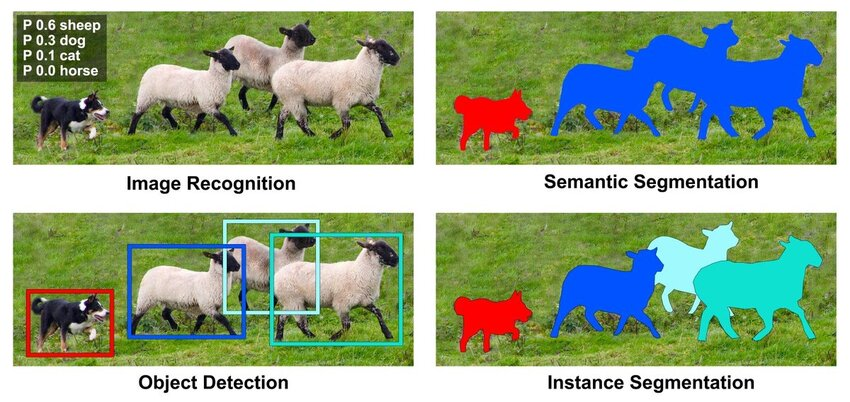
\includegraphics[width=0.9\textwidth]
    {figures/Comparison-of-image-classification-semantic-segmentation-and-semantic-instance.png}
    \caption{Comparison of image classification, object detection, semantic segmentation, and instance segmentation. Adapted from \citet{liu2022indoorscene}.}
    \label{fig:vision_task_comparison}
\end{figure}
Figure~\ref{fig:vision_task_comparison} illustrates the conceptual differences
between image classification, object detection, semantic segmentation, and instance
segmentation for visual perception tasks.


Based on findings in the literature and the requirements of interaction-point
detection, instance segmentation provides the most appropriate problem formulation
for this project. It allows individual buttons to be identified as distinct
entities while preserving pixel-level accuracy, which is essential for reliable
robotic interaction in dense and visually complex control interfaces. The
literature therefore clarifies the correct task formulation, but not yet which
model family best satisfies this requirement on embedded robotic hardware.


\section{Public datasets and annotation strategies.}

Public datasets for vision-based detection of elevator interfaces are limited, as
most indoor robotics datasets focus on navigation or scene understanding rather
than interaction elements \citep{sun2017scenenet}. This limits their direct
applicability to interaction-point perception tasks.

The IRSO 2018 dataset provides \gls{rgb} images of elevator panels captured in realistic
indoor environments and was originally introduced for object detection tasks
\citep{irso2018dataset}. Due to its focus on real elevator interfaces and visual
diversity, it is well suited for studying interaction-point perception in service
robotics.

Recent work reports a large-scale dataset with pixel-wise annotations for elevator
button segmentation \citep{liu2021elevator}. However, despite being described in the
literature, the corresponding semantic segmentation dataset is not publicly
available at the time this project is made and therefore cannot be used.

To enable instance-level interaction-point detection, this work reuses images from
the IRSO 2018 dataset and replaces the original annotations, namely
\gls{xml}-formatted bounding boxes and textual labels, with instance
segmentation masks. The new annotations are stored in the \gls{coco} format,
which supports instance-level labeling and is widely used across computer vision
frameworks, facilitating reuse and future extensions \citep{lin2014coco}. This
reveals a practical gap in the literature: relevant public images exist, but
publicly reusable instance-segmentation annotations for elevator interfaces are
still limited.

\section{Model design principles, evaluation metrics, and semantic interpretation}

Instance segmentation models for robotic perception typically follow a modular
design in which feature extraction, object localization, and pixel-level mask
prediction are handled by separate components within a single network. This design
enables shared visual representations while supporting accurate instance-level
localization, which is required for interaction-point perception in dense control
interfaces.

Region-based instance segmentation models such as \gls{maskrcnn} achieve high
localization accuracy through a two-stage design in which candidate regions are
proposed first and then refined by classification and mask-prediction heads
\citep{he2017maskrcnn}. This architecture is widely used as a reference and
benchmark in instance-segmentation research because of its strong instance-level
accuracy. However, its multi-stage processing increases computational cost and
memory use, which limits suitability for real-time deployment on embedded robotic
platforms.

To address these constraints, single-stage instance-segmentation architectures
have been developed that combine detection and mask prediction in a unified
pipeline. \gls{yolo}-based segmentation models, including the \gls{yolo}v8s
segmentation model, remain CNN-based vision models, but differ from
\gls{maskrcnn} in that they avoid a separate region-proposal stage and are
optimized for faster end-to-end inference \citep{jocher2023yolov8}. In practice,
this design trades some flexibility and, in some cases, peak segmentation
accuracy for substantially improved inference speed and computational efficiency,
which makes such models attractive for embedded robotic deployment.

Model performance is commonly evaluated using overlap-based metrics that measure
agreement between predicted masks and ground-truth annotations. \gls{iou} is defined as
\[
\mathrm{IoU} = \frac{|M_p \cap M_{gt}|}{|M_p \cup M_{gt}|},
\]
where $M_p$ and $M_{gt}$ denote the predicted and ground-truth masks. Average Precision
(\gls{ap}), computed over multiple \gls{iou} thresholds, is widely used as a standard evaluation
metric for instance segmentation tasks \citep{lin2014coco}.

For elevator-button perception, instance localization can be followed by a
recognition stage that determines the functional meaning of each detected button.
This can be achieved using character recognition, \gls{ocr}, or dedicated symbol
classification models applied to isolated button regions \citep{liu2021elevator}.
Accurate instance segmentation is a critical enabling step for such approaches, as
it provides clean, well-aligned inputs for subsequent classification or text
recognition.

In this work, instance segmentation is treated as the primary perception task, as
reliable instance-level localization is a prerequisite for any semantic
interpretation of interaction elements. The resulting pipeline is therefore
designed to support integration of \gls{ocr} or custom button classifiers, enabling the
robot to associate detected buttons with their intended functions in downstream
processing stages. The literature gives clear architectural candidates, but the
trade-off between multi-stage accuracy and single-stage deployability remains an
open design decision for this specific use case.

\section{Embedded deployment constraints in robotic perception}

Vision-based perception systems deployed on mobile service robots must operate
under strict computational and energy constraints. Prior work in robotic vision
reports that deep-learning models deployed on embedded platforms are limited by
onboard memory, processing power, and power consumption, which directly affects
real-time performance \citep{chen2018deeplearningrobots}.

Studies evaluating deep-learning inference on \gls{jetson}-class hardware show that
models achieving high accuracy on desktop \glspl{gpu} often exhibit increased latency and
memory usage when deployed on embedded devices \citep{kang2020edgeai}. These
findings indicate that benchmark accuracy alone is not a sufficient criterion for
model selection in robotic perception systems.

For instance segmentation tasks, this trade-off is particularly relevant, as mask
prediction introduces additional computational overhead compared to bounding-box
detection. Research on efficient model design highlights that architectural choices
such as backbone depth and feature reuse have a significant impact on inference
efficiency \citep{tan2019efficientnet}. Based on these insights, this project
treats model efficiency and deployability as primary design constraints alongside
segmentation accuracy.

Consequently, instance segmentation models considered in this work are evaluated
not only with respect to localization performance, but also in terms of their
suitability for embedded deployment. However, relatively few studies report this
trade-off for elevator-interface perception specifically. This literature-driven
perspective directly informs the model selection and optimization strategies
described in Chapter 3 (\nameref{ch:methodology}).

\section{Scalability, robustness, and reproducibility.}

Several studies emphasize that robust perception systems require more than a single
well-performing model. Instead, scalability is achieved through structured data
management, consistent annotation practices, and reproducible training pipelines
that support incremental dataset expansion and model updates
\citep{cordts2016cityscapes}. These practices reduce sensitivity to domain-specific
bias and enable adaptation to new environments without redesigning the entire
system.

From these findings, this project adopts a pipeline-oriented approach in which
dataset creation, annotation, training, and evaluation are treated as modular and
repeatable processes. Rather than optimizing a single model for a fixed dataset,
the focus is placed on maintaining a perception workflow that can be extended with
new data and retrained as deployment conditions evolve. Existing literature
strongly advocates reproducibility, but gives less attention to practical
feedback loops for environment-specific data collection and retraining after
deployment.


\section{Summary and identified research gap}

The reviewed literature shows that reliable perception of interaction elements in
robotic systems requires instance-level localization, suitable annotation
strategies, and awareness of embedded deployment constraints. Existing studies
demonstrate the technical feasibility of these components, but often address them
in isolation.

At the same time, publicly available datasets for elevator interfaces are limited,
and existing annotations are commonly designed for object detection rather than segmentation tasks. In addition, many approaches focus
on model performance without explicitly considering scalability, reproducibility,
or deployment on embedded robotic platforms.

This project addresses these gaps by repurposing a realistic elevator dataset with
instance-level annotations and by developing a scalable and deployment-aware
computer-vision pipeline for elevator-button perception in hospital environments.
The following chapter describes the methodology used to realize this approach.
